\documentclass{article}

\input{../../../preambule}
\usetikzlibrary{arrows}
\definecolor{wwqqtt}{rgb}{0.4,0,0.2}
\definecolor{zzttqq}{rgb}{0.6,0.2,0}
\definecolor{uququq}{rgb}{0.25,0.25,0.25}

\newtheorem{theorem}{Théorème}[subsection]

\hypersetup{colorlinks=true, urlcolor=bleu, linkcolor=red}

\begin{document}
Soient $H$ une sous-espace borné de $\mathbb{R}^+\backslash\{0\}$ pour lequel $0$ est un point d'accumulation, $\tilde{\Omega}$ un polygone ouvert de $\mathbb{R}^n$ tel que $\Omega\subset\tilde{\Omega}$ et, pour tout $h\in H$, on note $\tilde{\mathscr{T}}_h$ une triangulation sur $\tilde{\Omega}$ au moyen d'éléments $K$ dont le diamètre $h_K$ sont inférieurs ou égal à $h$ et soit $\tilde{V}_h$ un espace d'éléments finis construit sur $\tilde{\mathscr{T}}_h$ tel que :
\begin{equation} \label{eq5} \tilde{V}_h \text{ est un sous-espace de dimension fini de } H^m\left(\tilde{\Omega}\right)\cap C^k\left(\overline{\tilde{\Omega}}\right) \end{equation}
(voir fig. \ref{fig2})
\begin{figure}[!h]
\centering
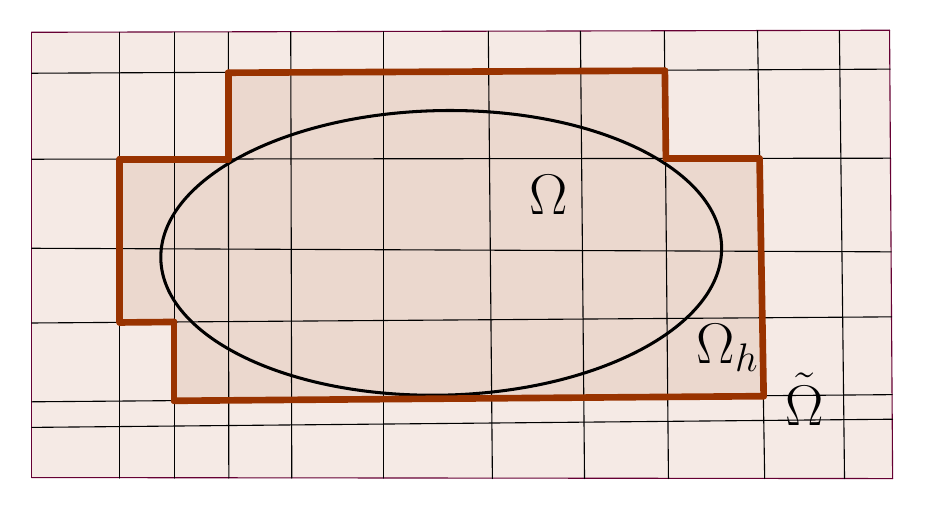
\begin{tikzpicture}[line cap=round,line join=round,>=triangle 45,x=1.0cm,y=1.0cm,scale=0.65]
\clip(3.82,-7.67) rectangle (20.82,1.26);
\fill[color=zzttqq,fill=zzttqq,fill opacity=0.1] (3.9,1.17) -- (20.66,1.21) -- (20.72,-7.55) -- (3.9,-7.53) -- cycle;
\fill[line width=2.4pt,color=zzttqq,fill=zzttqq,fill opacity=0.1] (7.74,-1.31) -- (7.74,0.38) -- (16.27,0.42) -- (16.29,-1.3) -- (18.12,-1.3) -- (18.2,-5.94) -- (6.68,-6.03) -- (6.68,-4.49) -- (5.62,-4.5) -- (5.62,-1.31) -- cycle;
\draw [line width=1.1pt, rotate around={1.21:(11.9,-3.14)}] (11.9,-3.14) ellipse (5.48cm and 2.78cm);
\draw [color=wwqqtt] (3.9,1.17)-- (20.66,1.21);
\draw [color=wwqqtt] (20.66,1.21)-- (20.72,-7.55);
\draw [color=wwqqtt] (20.72,-7.55)-- (3.9,-7.53);
\draw [color=wwqqtt] (3.9,-7.53)-- (3.9,1.17);
\draw (3.9,0.37)-- (20.67,0.45);
\draw (20.68,-1.29)-- (3.9,-1.31);
\draw (3.9,-3.05)-- (20.69,-3.12);
\draw (20.7,-4.39)-- (3.9,-4.51);
\draw (3.9,-6.05)-- (20.71,-5.91);
\draw (3.9,-6.55)-- (20.72,-6.39);
\draw (5.62,1.17)-- (5.62,-7.54);
\draw (6.68,-7.54)-- (6.68,1.17);
\draw (7.74,1.17)-- (7.75,-7.54);
\draw (8.98,-7.54)-- (8.96,1.18);
\draw (10.78,1.18)-- (10.78,-7.54);
\draw (12.9,-7.55)-- (12.82,1.19);
\draw (14.62,1.19)-- (14.7,-7.55);
\draw (16.34,-7.55)-- (16.26,1.19);
\draw (18.08,1.2)-- (18.22,-7.55);
\draw (19.78,-7.55)-- (19.68,1.2);
\draw [line width=2.4pt,color=zzttqq] (7.74,-1.31)-- (7.74,0.38);
\draw [line width=2.4pt,color=zzttqq] (7.74,0.38)-- (16.27,0.42);
\draw [line width=2.4pt,color=zzttqq] (16.27,0.42)-- (16.29,-1.3);
\draw [line width=2.4pt,color=zzttqq] (16.29,-1.3)-- (18.12,-1.3);
\draw [line width=2.4pt,color=zzttqq] (18.12,-1.3)-- (18.2,-5.94);
\draw [line width=2.4pt,color=zzttqq] (18.2,-5.94)-- (6.68,-6.03);
\draw [line width=2.4pt,color=zzttqq] (6.68,-6.03)-- (6.68,-4.49);
\draw [line width=2.4pt,color=zzttqq] (6.68,-4.49)-- (5.62,-4.5);
\draw [line width=2.4pt,color=zzttqq] (5.62,-4.5)-- (5.62,-1.31);
\draw [line width=2.4pt,color=zzttqq] (5.62,-1.31)-- (7.74,-1.31);
\begin{scriptsize}
\draw (14,-2) node {\huge{$\Omega$}};
\draw (17.5,-5) node{\huge{$\Omega_h$}};
\draw (19,-6) node{\huge{$\tilde{\Omega}$}};
\end{scriptsize}
\end{tikzpicture}
\caption{Définition des ensembles $\Omega$, $\tilde{\Omega}$ et $\Omega_h$ }
\label{fig2}
\end{figure}
\\
De plus, pour étudier la convergence de l'approximation, on suppose qu'il existe une famille d'opérateurs linéaires continus $(\tilde{\Pi}_h)_{h\in H}$ de $H^m(\Omega)$ dans $\tilde{V}_h$ satisfaisant :
\begin{equation} \label{eq6.1}
	\exists C>0;\ \forall h\in H,\ \forall l=0,...,m-1,\ \forall v\in H^m(\tilde{\Omega}),\ \left| v-\tilde{\Pi}_h v\right|_{l,\tilde{\Omega}}\leq Ch^{m-1}|v|_{m,\tilde{\Omega}}
\end{equation}
\begin{equation} \label{eq6.2}
	\forall v\in H^m(\tilde{\Omega}), \lim_{h\to 0} \left|v-\tilde{\Pi}_h v \right|_{m,\tilde{\Omega}}=0
\end{equation}
Ces conditions n'ont pas besoin de l'hypothèse classique de régularité de la méthode des éléments finis $H^m(\tilde{\Omega})\hookrightarrow C^s(\tilde{\Omega})$, où $s$ est l'ordre maximal des dérivés apparaissant dans la définition des degrés de liberté de l'élément fini générique de $(\tilde{V}_h)_{h\in H}$, mais on assume que :
\begin{equation} \label{eq7} \text{la famille } (\tilde{\mathscr{T}}_h)_{h\in H} \text{ est régulière} \end{equation}
Comme expliqué dans \cite{ciarlet72gal}, une famille est dite régulière si, en notant $h_K$ le diamètre de $K$ et $\rho_K$ le supremum du diamètre des sphères inscrites dans $K$ :
	\[\exists \alpha>0;\ \forall K\in\tilde{\mathscr{T}}_h,\ h_K\leq \alpha \rho_K\]
De plus, les conditions (\ref{eq6.1})-(\ref{eq6.2}) demandent l'hypothèse suivante : l'élément fini générique $(K,P_K,\Sigma_K)$ de la famille $(\tilde{V}_h)_{h\in H}$ statisfait l'équation $P_m(K)\subset P_K$ où $P_n(K)$ définit l'ensemble des polynômes de degré inférieur ou égal à $n$ définis sur $K$.

\bigskip
À présent, pour tout $h\in H$, on considère le sous-ensemble $\Omega_h$ (voir figure \ref{fig2}) définie par :
	\begin{equation} \label{eq8} \Omega_h \text{ est l'intérieur de l'union des rectangles } K \text{ de } \mathscr{T}_h \text{ tel que } K\cap\Omega\neq\emptyset \end{equation}
Il est clair que la famille $(\Omega_h)_{h\in H}$ satisfait les relations (en notant $\mu$ une mesure sur $\tilde{\Omega}$) :
\begin{eqnarray}
	\label{eq9} \forall h\in H, \Omega\subset\Omega_h\subset\tilde{\Omega}\\
	\label{eq10} \lim_{h\to 0} \mu(\Omega_h\backslash\overline{\Omega})=0
\end{eqnarray}
Pour tout $h\in H$, on définit :
	\begin{equation}\label{eq11} V_h=\{\restriction{\phi}{\Omega_h}| \phi\in\tilde{V}_h\}\end{equation}
Pour tout $\varepsilon>0$, on considère le problème de minimisation suivant : trouver $\sigma_{\varepsilon,h}^\eta\in V_h$ satisfaisant :
	\begin{equation} \label{eq12} \forall v_h\in V_h,\ J_{\varepsilon, h}^\eta (\sigma_{\varepsilon, h}^\eta)\leq J_{\varepsilon, h}^\eta (v_h) \end{equation}
où $J_{\varepsilon, h}^\eta$ est la fonctionnelle définie par :
	\[J_{\varepsilon, h}^\eta=\ell^\eta \left[(v_h-f)^2\right]+\varepsilon |v_h|^2_{m,\Omega_h}\]
On considère ensuite le problème variationnel suivant : trouver $\sigma_{\varepsilon,h}^\eta\in V_h$ satisfaisant :
	\begin{equation} \label{eq13} \forall v_h\in V_h,\ \ell^\eta (\sigma_{\varepsilon, h}^\eta v_h)+ \varepsilon \left(\sigma_{\varepsilon, h}^\eta,v_h\right)=\ell^\eta(fv_h) \end{equation}
où $(u,v)_{m,\Omega_h}=\sum_{|\alpha|=m} \int_{\Omega_h} \partial^\alpha u(x) \partial^\alpha v(x) dx$.\\

\begin{theorem}
On suppose que $\Omega$, $\omega$, $m$ et $f$ sont définis comme dans la section précédente et que les hypothèses (\ref{eq4}), (\ref{eq5}), (\ref{eq8}) et (\ref{eq11}) sont vérfiées. Alors, pour tout $\varepsilon>0$, tout $h\in H$, il existe $\eta_0>0$ tel que pour tout $\eta\in E$, $\eta\leq\eta_0$, les problèmes (\ref{eq12}) et (\ref{eq13}) admettent une même unique solution.
\end{theorem}

\begin{dem}
En utilisant un argument de compacité (voir \cite{necas67mthd}), on montre, sous la relation :
	\[\forall p\in P_{m-1}(\tilde{\Omega}_h),\ \restriction{p}{\omega}=0\Rightarrow p\equiv 0\]
que la fonction $[|\bullet|]_h$ définie sur $H^m(\Omega_h)$ par :
	\[[|v|]_h=\left(\|v\|^2_{0,\omega}+|v|_{m,\Omega_h}^2\right)^\frac{1}{2}\]
est une norme sur $H^m(\Omega_h)$ équivalente à la norme usuelle
	\[\|v\|_{m,\Omega_h}=\left( \sum_{|\alpha|\leq m} \int_{\Omega_h} (\partial^\alpha v)^2\right)^\frac{1}{2}\]
En conséquence de la définition de $\ell^\eta$, la forme bilinéaire symétrique :
	\[(u_h,v_h)\mapsto \ell^\eta(u_hv_h)+\varepsilon (u_h,v_h)_{m,\Omega_h}\]
est continue sur $V_h\times V_h$. Ainsi, la forme est $V_h$-elliptique pour tout $\eta$ assez petit car en utilisant (\ref{eq4}), on a :
\begin{equation}\label{eq14}
\begin{array}{c c l}
	\ell^\eta(v_h^2)+\varepsilon |v_h|^2_{m,\Omega_h} &\geq& \|v_h\|_{0,\omega}^2-C\eta^t \|v_h\|^2_{m,\Omega} + \varepsilon |v_h|^2_{m,\Omega_h}\\
							&\geq& \min(1,\varepsilon)\|v_h\|_h^2-C\eta^t \|v_h\|^2_{m,\Omega} \\
							&\geq& (C'\min(1,\varepsilon)-C\eta^t)\|v_h\|^2_{m,\Omega_h}
\end{array}
\end{equation}
où $C'$ est une constante liée à l'équivalence des normes.\\
Supposons (voir \cite{arcang04multidim} pour plus de détail) qu'il existe $\beta>0$ tel que, $\forall \varepsilon>0$, $\forall \eta\in E$, $\frac{\eta^t}{\min(1,\varepsilon)}<\beta$. En prenant $\beta=\frac{C'}{C}$, il existe $C''>0$ tel que \[\ell^\eta(v_h^2)+\varepsilon |v_h|^2_{m,\Omega_h}\geq C''\|v_h\|^2_{m,\Omega_h}\]
La forme est donc bilinéaire symétrique $V_h$-elliptique : le théorème de Lax-Milgram s'applique donc, et l'unicité de la solution est assurée.
\end{dem}

\begin{rmq}
En notant $M$ la dimension de $V_h$ et $(\phi_j)_{1\leq j\leq M}$ une base de $V_h$, on pose :
	\[\sigma_{\varepsilon, h}^\eta=\sum_{j=1}^M \alpha_j \phi_j\]
avec $\alpha_j\in\mathbb{R}$, $1\leq j\leq M$. On introduit les matrices :
	\[\mathcal{A}=\left(\ell^\eta (\phi_i\phi_j)\right)_{1\leq i,j\leq M}\] 
	\[\mathcal{R}=\left((\phi_i, \phi_j)_{m,\Omega_h}\right)_{1\leq i,j\leq M}\]
	\[\mathcal{F}=\left(\ell^\eta(f\phi_i)\right)_{1\leq i\leq M}\]
On voit que (\ref{eq13}) est équivalent au problème :
	\[\text{Trouver } (\alpha=(\alpha_1,...,\alpha_M)\in\mathbb{R}^M \text{ solution de } (\mathcal{A}+\varepsilon\mathcal{R})\alpha=\mathcal{F}\]
On peut enfin prendre comme approximation de $f$ la fonction $\Phi=\restriction{\sigma_{\varepsilon,h}^\eta}{\Omega}$ qui, en utilisant les hypothèses (\ref{eq5}), (\ref{eq8}) et (\ref{eq11}), appartient à $H^m(\Omega)\cap C^k(\overline{\Omega})$.\\
On cherche à savoir en quel sens $\Phi$ est une approximation de $f$.
\end{rmq}

\begin{theorem}
Sous les mêmes hypothèses, si on suppose de plus que (\ref{eq6}) est vérifié, alors la solution $\sigma_{\varepsilon,h}^\eta$ de (\ref{eq12}) et (\ref{eq13}) satifont :
\begin{enumerate}
	\item \[\lim_{\substack{\varepsilon\to 0\\ \frac{h^{2m}}{\varepsilon}\to 0 \\ \frac{\eta^t}{\varepsilon}\to 0}} \|\sigma^\eta_{\varepsilon, h}-\sigma\|_{m,\Omega}=0\]
où $\sigma$ est la solution de (\ref{eq1}) et où $\beta$ a été introduit dans le théorème précédent
	\item Il existe une constante positive $C$ telle que :
		\[\|\sigma_{\varepsilon, h}^\eta - f\|_{0,\omega}^2\leq C\left(h^{2m}+\eta^t o(1)+\varepsilon\right) \text{ où } \varepsilon\to 0, \frac{h^{2m}}{\varepsilon}\to 0, \frac{\eta^t}{\varepsilon}<\beta\]
\end{enumerate}
\end{theorem}

\begin{dem}
Soit $\sigma$ l'unique solution de (\ref{eq1}). On a $\restriction{\sigma}{\omega}=\restriction{f}{\omega}$ et
	\[\|\sigma_{\varepsilon,h}^\eta -f\|_{0,\omega}^2=\|\sigma_{\varepsilon,h}^\eta -\sigma\|_{0,\omega}^2\]
On a, en utilisant (\ref{eq4}) : 
\begin{equation} \label{eq15} \|\sigma_{\varepsilon,h}^\eta -f\|_{0,\omega}^2\leq \ell^\eta \left( \left(\sigma_{\varepsilon, h}^\eta -\sigma\right)^2\right) + C\eta^t \|\sigma_{\varepsilon, h}^\eta -\sigma\|_{m,\Omega}^2 \end{equation}
D'où, de (\ref{eq12}), on a :

\begin{equation} \label{eq16} \forall v_h\in V_h,\ \ell^\eta\left( \left(\sigma_{\varepsilon, h}^\eta -\sigma\right)^2\right) + \varepsilon |\sigma^\eta_{\varepsilon, h}|^2_{m,\Omega_h}\leq \ell^\eta \left( \left(v_h -\sigma\right)^2\right) + \varepsilon |v_h|^2_{m,\Omega_h} \end{equation}

\end{dem}

\bibliographystyle{plain}
\bibliography{bib}
\end{document}
